\section{System Model}\label{sec_system}
The system model consists of three parts: a software application, an execution platform, and a software allocation scheme. An overview of the system model is illustrated in Figure \ref{fig_softwareallocation}. The software application is a user-defined software system, such as x-by-wire, electronic throttle control, flight control, etc., which is developed using software components \cite{softwarecomponents}\cite{Crnkovic2002BuildingSystems}. The application is deployed on an execution platform, which is a network of heterogeneous nodes with possibly different processor frequencies, power consumption, and failure-rates. The allocation scheme, which defines a mapping relation from software components to computational nodes, guarantees that the extra-functional properties such as application reliability and timing requirements are met. Furthermore, it takes the optimization of power consumption as its objective in the allocation process.
\begin{figure}[!h]
\centering
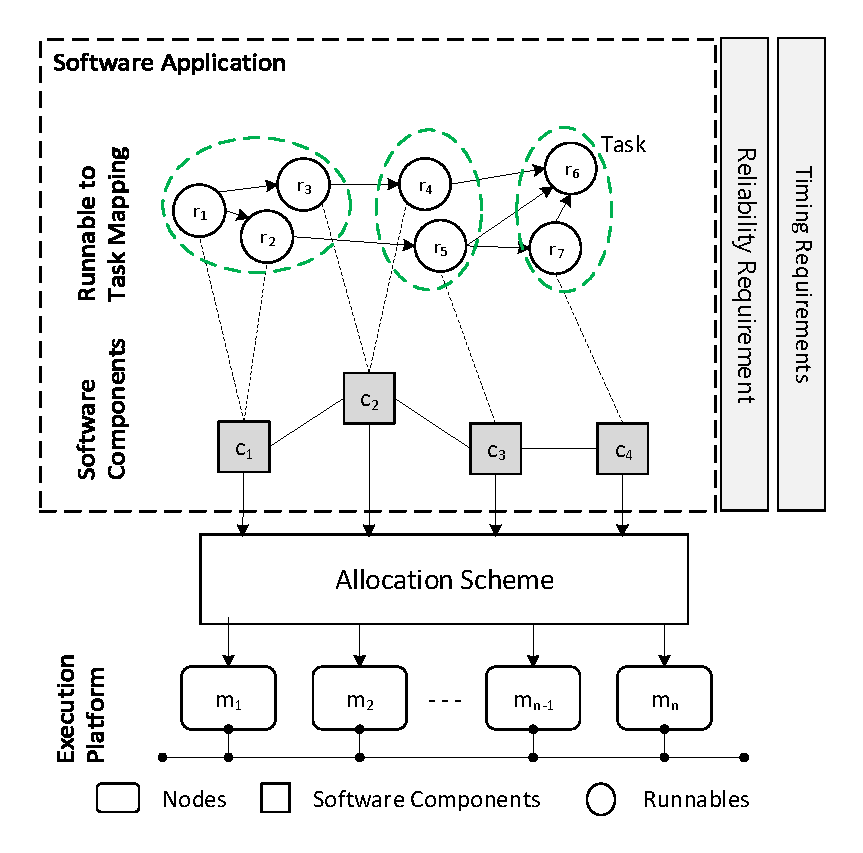
\includegraphics[scale=0.6]{softwareallocation}
\caption{System Model.}
\label{fig_softwareallocation}
\end{figure}

In this work, we target AUTOSAR-based systems due to the increasing popularity of the specification standard in  the automotive industry, and the challenges and opportunities that automotive industry is facing especially in resource optimization and dependability of automotive systems. Note that our approach can also be applied on different domains of distributed embedded systems with a slight change in the application modeling.

\subsection{Software Application Model}
In AUTOSAR-based systems, a software application is developed using AUTOSAR application software components $C$ that consist of one or more runnables $R_c$~\cite{Schreiner2007ABus}. In this notation, $R_{c_i}$ refers to the set of runnables that are co-hosted in the component $C_i$.
\begin{definition}[Software Application] We define an AUTOSAR software application $\zeta$ as a \textit{Digraph} (acyclic directed graph) $\langle V_r, E\rangle$ of runnable nodes $V_r$, where $\langle u,v\rangle\in E$ is a set of directed links from $u$ to $v$, which denote the logical flow of the application, and $u,v\in V_r$. The runnable is a tuple $\langle e, p \rangle$, where $\bigcup_{i=1}^{N} e_{i}$ is a set of execution times, $p$ is a periodic activation, and $e_i$ refers to the execution time of the runnable $r$ on the node $m_i$.
\end{definition}
 
The following assumptions are made in our proposed software allocation method:
\begin{itemize}
\item Allocatable software components are considered atomic, and therefore are allocated only on a single node, whereas, composite components need to be flattened first into their respective constituents of atomic components.
\item Runnables are activated either periodically by clock events, or by predecessor runnables.
\item Three cases of mapping runnables to tasks are considered: i) a runnable is mapped to a single task, ii) runnables that are collocated on the same software component are mapped to a single task, iii) runnables with the same activation periods and with triggering dependency are mapped to a single task. For more information, please see the AUTOSAR documentation \cite{AUTOSAR2017SpecificationSoftware}.
\item We assume that the computation nodes have the same types of interfaces. If this is not the case, software components can be constrained to nodes that the component supports.
\end{itemize}

\subsection{Fault-tolerant Software Application Model}
Redundancy is the most common way to increase the reliability of an application. It can be implemented according to different schemes, such as hot stand-by, cold stand-by, etc~\cite{Dubrova2013Fault-tolerantDesign}. In this work the details of the redundancy scheme are abstracted away under the following assumptions: i) Hot stand-by redundancy technique is used for the replacement of failed components, which are identical and are allocated on different nodes, ii) software components need to be replicated if the application's reliability requirement is not met without replication, otherwise they are not replicated, iii) the time needed to detect and replace a faulty component is considered negligible and will not be taken into account in the response time analysis of tasks and delay calculation of cause-effect chains, iv) Because of its simplicity, the mechanism for detection and replacement of faulty components will be considered fault-free, and therefore will not be included in the reliability calculations.

We denote the $k^{th}$ replica of a software component $c$ as $c^k$, with $1\le k\leq K$; where $K$ is the maximum number of replicas allowed for each application component.

\subsection{Platform Model}
The application is deployed on a network of heterogeneous computing nodes that are connected via a reliable communication network, the CAN bus. The computation node is specified as a 3-tuple $\langle hz, \lambda, p \rangle$, respectively, refer to the processor frequency, failure-rate and power consumption of a computation node. Due to the heterogeneity assumption of the processors, an application maybe be deployed on nodes with higher processor frequencies, and therefore fewer number of nodes in order to minimize the total power consumption of the system. However, due to the application reliability requirement, the application could be deployed differently, and with more resources. The CAN bus is considered reliable, for instance through redundancy. Therefore, its exclusion from the overall calculation of the system's reliability does not impact our proposed software allocation. %Figure~\ref{fig_softwareallocation} illustrates an overview of an AUTOSAR software application deployment on a set of computational nodes via a software allocation scheme that is discussed in Section~\ref{sec_allocation}.

